\documentclass[journal,12pt,twocolumn]{IEEEtran}
\usepackage{cite}
\usepackage{amsmath,amssymb,amsfonts,amsthm}
\usepackage{algorithmic}
\usepackage{graphicx}
\usepackage{textcomp}
\usepackage{xcolor}
\usepackage{txfonts}
\usepackage{listings}
\usepackage{enumitem}
\usepackage{mathtools}
\usepackage{gensymb}
\usepackage{comment}
\usepackage[breaklinks=true]{hyperref}
\usepackage{tkz-euclide}
\usepackage{gvv}
\def\inputGnumericTable{}
\usepackage[latin1]{inputenc}
\usepackage{color}
\usepackage{array}
\usepackage{longtable}
\usepackage{calc}
\usepackage{multirow}
\usepackage{hhline}
\usepackage{ifthen}
\usepackage{lscape}

\newtheorem{theorem}{Theorem}[section]
\newtheorem{problem}{Problem}
\newtheorem{proposition}{Proposition}[section]
\newtheorem{lemma}{Lemma}[section]
\newtheorem{corollary}[theorem]{Corollary}
\newtheorem{example}{Example}[section]
\newtheorem{definition}[problem]{Definition}
\newcommand{\BEQA}{\begin{eqnarray}}
\newcommand{\EEQA}{\end{eqnarray}}
\newcommand{\define}{\stackrel{\triangle}{=}}
\theoremstyle{remark}
\newtheorem{rem}{Remark}

\begin{document}

\bibliographystyle{IEEEtran}
\title{Gate 2023 EC 58}
\author{HIBA MUHAMMED\\
        EE23BTECH11026}
\maketitle

\section*{Problem Statement}
Let $x_1(t) = u(t + 1.5) - u(t - 1.5)$ and $x_2(t)$ is shown in the figure below. For $y(t) = x_1(t) * x_2(t)$, the $\int_{-\infty}^{\infty} y(t) \, dt$ is \underline{\hspace{2cm}}.

\begin{figure}[htbp]
    \centering
    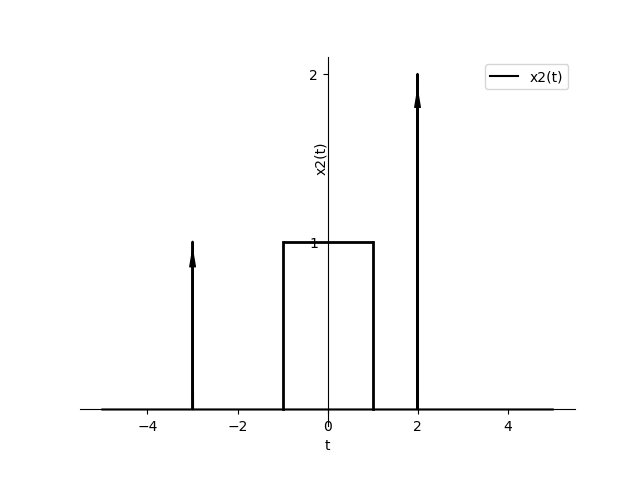
\includegraphics[width=0.5\textwidth]{gatefig.png}
    \caption{Figure}
    \label{fig:graph}
\end{figure}

\section*{Solution}
\section*{Input Parameters}
\begin{table}[htbp]
    \centering
    \begin{tabular}{|c|c|p{6cm}|}
        \hline
        \multicolumn{3}{|c|}{\textbf{Input Parameters}} \\
        \hline
        \textbf{Function} & \textbf{Expression} & \textbf{Description} \\
        \hline
        $x_1(t)$ & $u(t + 1.5) - u(t - 1.5)$ & Step function with delay and width parameters. \\
        $x_1(\omega)$ & $3\text{sinc}(1.5\omega)$ & Fourier Transform of $x_1(t)$. \\
        $x_2(t)$ & $\delta(t + 3) + \text{rect}\left(\frac{t}{2}\right) + 2\delta(t - 2)$ & Impulse function followed by a rectangle and two impulses. \\
        $x_2(\omega)$ & $e^{3j\omega} + 2\text{sinc}(\omega) + 2e^{-2j\omega}$ & Fourier Transform of $x_2(t)$. \\
        \hline
    \end{tabular}
\end{table}


\begin{flalign*}
& x_1(t) = u(t+1.5) - u(t-1.5) & \\
& x_1(t) = \text{rect}\left(\frac{t}{3}\right) & \\
& x_1(t) = \text{recr}\left(\frac{t}{3}\right)&\\ 
& \text{rect}(t) = \text{rect}\left(\frac{t}{a}\right) \longleftrightarrow a \cdot \text{sinc}(a\omega) &\\
& X1(\omega)=3\text{sinc}(1.5\omega) & \\
& x_2(t) = \delta(t+3) + \text{rect}\left(\frac{t}{2}\right) + 2\delta(t-2) & \\
& X_2(\omega) = e^{3j\omega} + 2\text{sinc}(\omega) + 2e^{-2j\omega} & \\
& y(t) = x_1(t) * x_2(t) & \\
& Y(\omega) = X_1(\omega) \cdot X_2(\omega) & \\
& \text{We know:} & \\
& Y(\omega) = \int_{-\infty}^{\infty} y(t)e^{-j\omega t} dt & \\
& \int_{-\infty}^{\infty} y(t) = Y(0) & \\
& Y(0) = X_1(0) \cdot X_2(0) & \\
& \quad = 3(1+2+2) & \\
& \quad = 15 &
\end{flalign*}

\end{document}

